\chapter{Viewpoints}
\label{chap:viewpoints}

In dit hoofdstuk worden \emph{design viewpoints} besproken die relevant voor het systeem zijn. 
Naarmate de ontwikkelingen van CalZone vorderen, zullen deze viewpoints uitgebreid worden en eventueel aangepast worden. 
Op het einde van de laatste iteratie wordt verwacht dat alle requirements uit het SRS van dit project ontworpen zijn. 
Voorlopig wordt er in de volgende secties enkel het design besproken van deze eerste iteratie.

\section{Context}
\label{sec:context}

De gebruikers van het systeem zijn onder te verdelen in 5 categori\"{e}n: externen, studenten, professoren, assistenten en programmabeheerders. 
Elk soort gebruiker moet in de finale versie van CalZone in staat zijn de functionaliteiten die specifiek aan deze gebruikers zijn toegekend toe te passen. 
\\
In de huidige fase van het project is er nog geen onderscheid te merken in de verschillende soorten gebruikers naar de buitenwereld toe, hoewel er in de databank wel reeds rekening mee is gehouden (zie sectie~\ref{sec:data}). 
Daarom wordt er voortaan in deze tekst enkel over gebruikers in zijn meest algemene vorm gesproken.
\\
Gebruikers zijn in staat om zich te registreren in het systeem. 
Hierdoor kunnen ze inloggen en bezitten deze gebruikers een profielpagina. 

\begin{figure}[H]
	\centering
	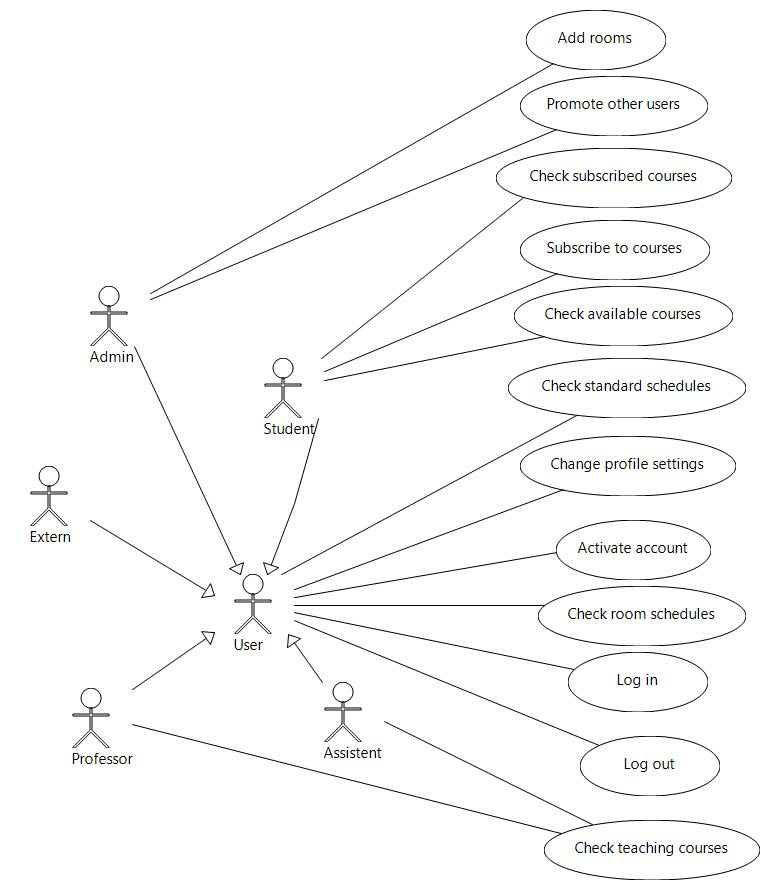
\includegraphics[scale=0.5]{design/papyrus/use_cases.jpg}
	\label{fig:usecase}
	\caption{Use case diagram}
\end{figure}

\section{Logica}
\label{sec:logica}

In deze sectie worden de verschillende modules en packages behandeld die tesamen het huidige systeem vormen.

\subsection{Controllers}
\label{subsec:controllers}

Deze klassen zijn verantwoordelijk om de HTTP-requests te verwerken. 
Deze klassen zorgen dus voor een propagatie van (functionaliteits)verzoeken van de front-end naar de back-end. 
Eveneens zorgen deze klassen ook voor een propagatie van data van de back-end naar de front-end. 
Dit laatste uit zich in het voorzien van webpagina's.
Met andere woorden zorgen de controllers dus voor de mogelijke views en voorzien dus de mogelijkheid om de functionaliteiten opgesomd in het use case diagram van sectie~\ref{sec:context} uit te voeren. 
Voor volgende concepten zijn er nu controllers voorzien:

\begin{itemize}
	\item Login
	\item Profieloverzicht
	\item Registratie
	\item Accountactivatie
\end{itemize}

\subsection{Databaseklassen}
\label{subsec:databaseklassen}

CalZone maakt gebruik van een relationele databank, MySQL, als back-end voor dataopslag. 
Om informatie vanuit deze databank te lezen en er naartoe te schrijven zijn er enkele klassen voorzien die een abstractie bieden voor het openen en sluiten van de connectie met de databank en het sturen van queries naar de databank. 
Volgende klassen zijn hiervoor voorzien:

\begin{itemize}
	\item DbConfig: Deze klasse voorziet de mogelijkheid om gegevens op te halen om toegang te kunnen krijgen tot een bepaalde databank. 
	Deze gegevens de gebruikersnaam, het wachtwoord en de locatie van de databank. 
	\item DbLink: Het openen en sluiten van de databankconnecties samen met het sturen van queries en het ontvangen van resultaten.
	\item DbTranslate: Een collectie van methodes die gemapt worden op queries
\end{itemize} 

\subsection{Data Access Objects}
\label{subsec:dao}

Het ophalen van data uit de MySQL databank gebeurt via \emph{Data Access Objects} of kortweg DAO's. 
Deze objecten gebruiken de algemene databasemethoden voorzien door de databaseklassen aangehaald in subsectie~\ref{subsec:databaseklassen} om specifieke data op te halen uit de databank en in te laden in het systeem. 
Ook wordt specifieke informatie via deze DAO's weggeschreven naar de databank. 
Volgende DAO's zijn aangemaakt in deze iteratie:

\begin{itemize}
	\item ActivationKeyDao: de activatiesleutels gebonden aan een geregisteerd account. 
	\item UserDao: gebruikergegevens
	\item SessionDao: gebruikerssessies met het systeem.
\end{itemize}

\subsection{Validators}
\label{subsec:validators}

Binnenin het systeem dient sommige data gecontroleerd te worden op geldigheid. 
Deze validatorklassen zijn verantwoordelijk om geldigheid van bepaalde informatie te controleren en aan te geven indien deze info niet geldig is. 
Volgende validators zijn in het huidige systeem aanwezig:

\begin{itemize}
	\item Email: controle op het emailadres
	\item Gebruikers: controle op de gebruikersnaam om profiel
\end{itemize}

\section{Data}
\label{sec:data}

De huidige databank is ontworpen om gebruikers, die zich willen registreren in het systeem, op te slaan. 
Men maakt een onderscheid tussen gebruikers die al dan niet hun account geactiveerd hebben. 
Een gebruiker die niet geactiveerd is, bezit een lijst van activatiesleutels. 
Dit is een lijst omdat activatiesleutels slechts tijdelijk geldig zijn en gebruikers in staat moeten kunnen zijn om een nieuwe activatiesleutel aan te vragen indien ze hun account als dan nog willen activeren nadat hun huidige activatiesleutel vervallen is.
Geactiveerde gebruikers kunnen inloggen. 
Hierdoor wordt een sessie aangemaakt in het systeem. 
Deze sessies worden gelogd in de databank. Figuur~\ref{fig:EER diagram} toont het EER-model van de databank.

\begin{figure}[H]
	\centering
	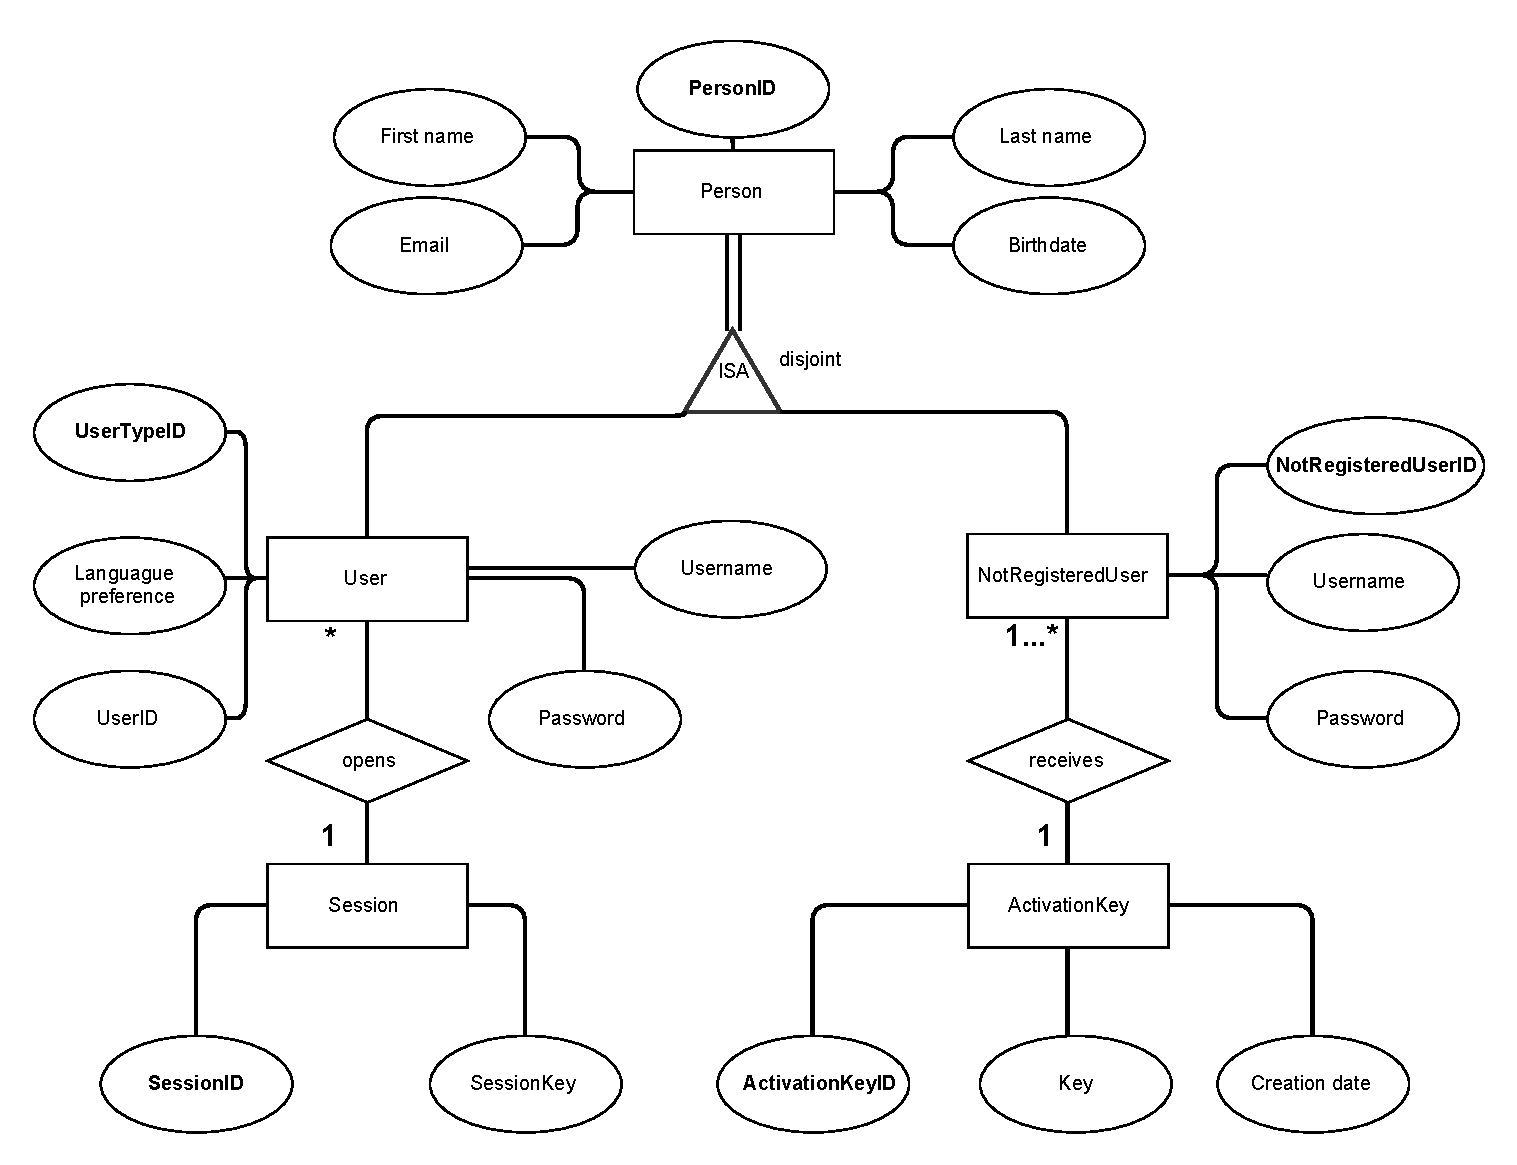
\includegraphics[scale=0.5]{design/EERIT1.pdf}
	\caption{EER diagram}
	\label{fig:EER diagram}
\end{figure}